\documentclass[aspectratio=169,10pt]{beamer}

\usepackage{array}
\usepackage{booktabs}
\usepackage{graphicx}
\usepackage{amsmath}
\usepackage{amssymb}
\usepackage{tikz}
\usetikzlibrary{arrows.meta,calc,positioning,shapes.geometric,fit}
\newcolumntype{L}[1]{>{\raggedright\arraybackslash}p{#1}}

% DGIST ISL Custom Color Palette
\definecolor{islteal}{RGB}{43,133,147}
\definecolor{islred}{RGB}{203,76,65}
\definecolor{isldark}{RGB}{52,61,67}
\definecolor{islnavy}{RGB}{31,55,95}
\definecolor{islmuted}{RGB}{92,101,108}
\definecolor{isllight}{RGB}{236,241,243}
\definecolor{islgold}{RGB}{184,119,20}
\definecolor{islgreen}{RGB}{44,145,91}
\definecolor{islpurple}{RGB}{130,58,160}

\newcommand{\deckdate}{2026.08.21}
\newcommand{\labname}{DGIST Intelligent Systems and Learning Laboratory}

\setbeamersize{text margin left=0.65cm,text margin right=0.65cm}
\setbeamertemplate{navigation symbols}{}
\setbeamertemplate{blocks}[rounded][shadow=false]
\setbeamercolor{normal text}{fg=isldark,bg=white}
\setbeamercolor{frametitle}{fg=isldark,bg=white}
\setbeamercolor{footer}{fg=white,bg=isldark}
\setbeamerfont{frametitle}{series=\bfseries,size=\Large}
\setbeamerfont{normal text}{size=\small}

\setbeamertemplate{frametitle}{%
  \nointerlineskip%
  \begin{beamercolorbox}[wd=\paperwidth,ht=1.35cm,dp=0cm]{frametitle}
    \vskip0.45cm%
    \hspace*{0.74cm}\insertframetitle\par%
    \vskip0.05cm%
    \hspace*{0.74cm}{\color{islteal}\rule{0.68\paperwidth}{4pt}}%
    {\color{islred}\rule{0.20\paperwidth}{4pt}}%
  \end{beamercolorbox}%
}

\setbeamertemplate{footline}{%
  \leavevmode%
  \begin{beamercolorbox}[wd=\paperwidth,ht=0.34cm,dp=0.11cm]{footer}
    \hspace*{0.65cm}{\scriptsize\deckdate}%
    \hfill{\scriptsize Reinforcement Learning \& Robotics Track \quad $\vert$ \quad Week 01: MDPs \& Baselines}\hfill%
    {\scriptsize\insertframenumber\,/\,\inserttotalframenumber}\hspace*{0.65cm}%
  \end{beamercolorbox}%
}

\newcommand{\bottomrulebar}{%
  \begin{tikzpicture}[remember picture,overlay]
    \fill[islteal] (current page.south west) rectangle ++(0.43\paperwidth,0.11cm);
    \fill[isldark] ([xshift=0.43\paperwidth]current page.south west)
      rectangle ++(0.34\paperwidth,0.11cm);
    \fill[islred] ([xshift=0.77\paperwidth]current page.south west)
      rectangle ++(0.23\paperwidth,0.11cm);
  \end{tikzpicture}%
}

\newcommand{\sectionlabel}[1]{%
  {\small\bfseries\color{islteal}#1}\par\vspace{0.14cm}%
}

\begin{document}

% ==========================================
% SLIDE 1: Title Slide
% ==========================================
\begin{frame}[plain,noframenumbering]
  \bottomrulebar
  \vspace{1.00cm}
  {\centering
    {\fontsize{22}{26}\selectfont\bfseries\color{islnavy}
      Week 01: MDPs, Rollouts, and Baselines\par}
    \vspace{0.22cm}
    {\fontsize{15}{18}\selectfont\color{islteal}
      The Foundations of Controlled Interaction Under Uncertainty\par}
    \vspace{0.50cm}
    {\large\bfseries Reinforcement Learning \& Robot Learning Core Curriculum\par}
    \vspace{0.20cm}
    {\small Presented by \textbf{DGIST ISL Team}\par}
    \vspace{0.12cm}
    {\small\color{islmuted} \labname\par}
    \vspace{0.10cm}
    {\small \deckdate\par}
    \vspace{0.45cm}
    {\scriptsize\color{islmuted}
      Core Concepts: MDP Tuple $\cdot$ Agent-Environment Loop $\cdot$ Episode Return $\cdot$ Random Baseline\par}
  }
\end{frame}

% ==========================================
% SLIDE 2: The Agent-Environment Interface
% ==========================================
\begin{frame}{The Agent-Environment Interface \& MDP Tuple}
  \sectionlabel{Reinforcement learning is structured sequential decision-making}

  {\centering
    \begin{tikzpicture}[
      box/.style={rounded corners=4pt, text width=6.5cm, minimum height=2.8cm, inner sep=5pt, font=\scriptsize, line width=0.9pt, align=left}
    ]
      % Left Card: Interface Loop
      \node[box, draw=islteal, fill=islteal!6] at (3.5, 1.5) {
        {\bfseries\color{islteal}\normalsize The Interaction Loop}\\[2pt]
        $\bullet$ \textbf{Agent:} Observes state $s_t$, selects action $a_t \sim \pi(\cdot|s_t)$.\\[1pt]
        $\bullet$ \textbf{Environment:} Emits next state $s_{t+1}$, reward $r_t$, and ending signals.\\[1pt]
        $\bullet$ Agent controls \textit{actions}; environment governs \textit{dynamics}.
        \vskip2pt
        \centering
        \begin{tikzpicture}[scale=0.55]
          \draw[thick, islnavy, fill=islnavy!15, rounded corners=2pt] (0,0.8) rectangle (1.8,1.5) node[pos=.5]{\tiny \textbf{Agent}};
          \draw[thick, isldark, fill=isllight, rounded corners=2pt] (0,-0.7) rectangle (1.8,0.0) node[pos=.5]{\tiny \textbf{Environment}};
          \draw[-{Latex}, thick, islred] (1.8,1.15) -- (2.5,1.15) -- (2.5,-0.35) -- (1.8,-0.35) node[pos=0.5, right]{\tiny $a_t$};
          \draw[-{Latex}, thick, islteal] (0,-0.35) -- (-0.7,-0.35) -- (-0.7,1.15) -- (0,1.15) node[pos=0.5, left]{\tiny $s_{t+1}, r_t$};
        \end{tikzpicture}
      };

      % Right Card: MDP Formalism
      \node[box, draw=islnavy, fill=islnavy!6] at (10.7, 1.5) {
        {\bfseries\color{islnavy}\normalsize The Formal MDP Tuple: $\mathcal{M} = (\mathcal{S}, \mathcal{A}, \mathcal{P}, \mathcal{R}, \gamma)$}\\[2pt]
        $\bullet$ $\mathcal{S}$: State space (discrete positions or continuous poses).\\[1pt]
        $\bullet$ $\mathcal{A}$: Action space (discrete commands or motor torques).\\[1pt]
        $\bullet$ $\mathcal{P}(s'|s, a)$: Transition probability function.\\[1pt]
        $\bullet$ $\mathcal{R}(s, a, s')$: Reward function mapping steps to scalar feedback.\\[1pt]
        $\bullet$ $\gamma \in [0, 1]$: Discount factor prioritizing near-term rewards.
      };
    \end{tikzpicture}
  \par}
\end{frame}

% ==========================================
% SLIDE 3: Anatomy of an RL Rollout
% ==========================================
\begin{frame}{Anatomy of an Episode Rollout \& Trajectory}
  \sectionlabel{How step-level transitions aggregate into total episode return}

  {\centering
    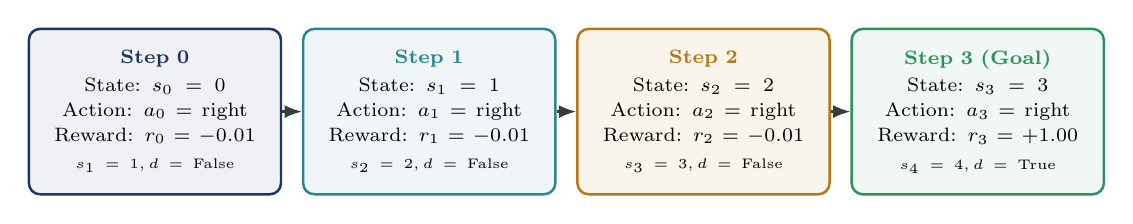
\begin{tikzpicture}[
      node distance=0.25cm,
      stage/.style={rounded corners=4pt, text width=2.85cm, minimum height=2.1cm, align=center, inner sep=5pt, font=\scriptsize, line width=0.9pt},
      arr/.style={-{Latex[length=2.2mm]}, thick, color=isldark}
    ]
      \node[stage, draw=islnavy, fill=islnavy!7] (s0) {
        {\bfseries\color{islnavy} Step 0}\\[2pt]
        State: $s_0 = 0$\\[1pt]
        Action: $a_0 = \text{right}$\\[1pt]
        Reward: $r_0 = -0.01$\\[2pt]
        \tiny $s_1 = 1, d = \text{False}$
      };

      \node[stage, draw=islteal, fill=islteal!7, right=of s0] (s1) {
        {\bfseries\color{islteal} Step 1}\\[2pt]
        State: $s_1 = 1$\\[1pt]
        Action: $a_1 = \text{right}$\\[1pt]
        Reward: $r_1 = -0.01$\\[2pt]
        \tiny $s_2 = 2, d = \text{False}$
      };

      \node[stage, draw=islgold, fill=islgold!8, right=of s1] (s2) {
        {\bfseries\color{islgold} Step 2}\\[2pt]
        State: $s_2 = 2$\\[1pt]
        Action: $a_2 = \text{right}$\\[1pt]
        Reward: $r_2 = -0.01$\\[2pt]
        \tiny $s_3 = 3, d = \text{False}$
      };

      \node[stage, draw=islgreen, fill=islgreen!7, right=of s2] (s3) {
        {\bfseries\color{islgreen} Step 3 (Goal)}\\[2pt]
        State: $s_3 = 3$\\[1pt]
        Action: $a_3 = \text{right}$\\[1pt]
        Reward: $r_3 = +1.00$\\[2pt]
        \tiny $s_4 = 4, d = \text{True}$
      };

      \draw[arr] (s0) -- (s1);
      \draw[arr] (s1) -- (s2);
      \draw[arr] (s2) -- (s3);
    \end{tikzpicture}
  \par}

  \vspace{0.14cm}
  \begin{columns}[T,onlytextwidth]
    \column{0.48\textwidth}
      \begin{block}{\small\color{islteal}\textbf{Undiscounted Return: $G = \sum_{t=0}^T r_t$}}
        \footnotesize $G = (-0.01) + (-0.01) + (-0.01) + (+1.00) = \mathbf{+0.97}$. Negative step costs penalize hesitation.
      \end{block}
    \column{0.48\textwidth}
      \begin{block}{\small\color{islnavy}\textbf{Discounted Return: $G = \sum_{t=0}^T \gamma^t r_t$}}
        \footnotesize For $\gamma = 0.90$: $G = -0.01 - 0.01(0.9) - 0.01(0.81) + 1.00(0.729) = \mathbf{+0.7019}$.
      \end{block}
  \end{columns}
\end{frame}

% ==========================================
% SLIDE 4: LineWorld Minimal Specification
% ==========================================
\begin{frame}{The LineWorld Benchmark Environment}
  \sectionlabel{A minimal 1D discrete MDP for rigorous baseline comparison}

  {\centering
    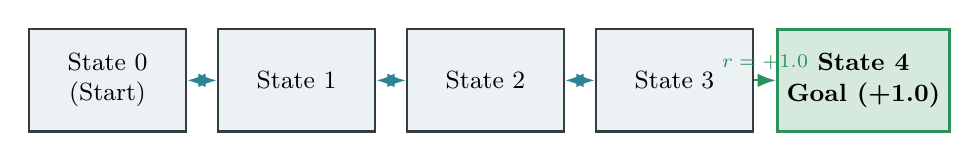
\begin{tikzpicture}[
      cell/.style={rectangle, draw=isldark, fill=isllight, minimum width=2.0cm, minimum height=1.3cm, align=center, font=\small, line width=0.8pt},
      goal/.style={rectangle, draw=islgreen, fill=islgreen!20, minimum width=2.0cm, minimum height=1.3cm, align=center, font=\small\bfseries, line width=1.1pt}
    ]
      \node[cell] (c0) at (0,0) {State 0\\(Start)};
      \node[cell] (c1) at (2.4,0) {State 1};
      \node[cell] (c2) at (4.8,0) {State 2};
      \node[cell] (c3) at (7.2,0) {State 3};
      \node[goal] (c4) at (9.6,0) {State 4\\Goal (+1.0)};

      \draw[{Latex}-{Latex}, thick, islteal] (c0) -- (c1);
      \draw[{Latex}-{Latex}, thick, islteal] (c1) -- (c2);
      \draw[{Latex}-{Latex}, thick, islteal] (c2) -- (c3);
      \draw[-{Latex}, thick, islgreen] (c3) -- (c4) node[midway, above]{\scriptsize $r=+1.0$};
    \end{tikzpicture}
  \par}

  \vspace{0.25cm}
  \begin{columns}[T,onlytextwidth]
    \column{0.48\textwidth}
      {\small\bfseries\color{islteal} MDP Rules}\par\vspace{0.06cm}
      {\footnotesize
      $\bullet$ $\mathcal{S} = \{0, 1, 2, 3, 4\}$, start state $s_0 = 0$.\\[2pt]
      $\bullet$ $\mathcal{A} = \{0: \text{left}, 1: \text{right}\}$.\\[2pt]
      $\bullet$ Boundaries: moving left at $s=0$ stays at $s=0$.\\[2pt]
      $\bullet$ Step cost: $r = -0.01$ for every non-goal transition.}

    \column{0.48\textwidth}
      {\small\bfseries\color{islnavy} Termination Signals}\par\vspace{0.06cm}
      {\footnotesize
      $\bullet$ \textbf{Terminated ($d_{\text{term}}$):} Reaching goal state $4$ ($r = +1.00$).\\[2pt]
      $\bullet$ \textbf{Truncated ($d_{\text{trunc}}$):} Exceeding maximum horizon $T_{\max} = 20$.\\[2pt]
      $\bullet$ Clear distinction between task success and horizon timeout.}
  \end{columns}
\end{frame}

% ==========================================
% SLIDE 5: The Role of Baselines
% ==========================================
\begin{frame}{The Role of Baselines in Reinforcement Learning}
  \sectionlabel{Why random and heuristic baselines are required before claiming learning success}

  \renewcommand{\arraystretch}{1.20}
  \setlength{\tabcolsep}{6pt}
  {\centering
    \footnotesize
    \begin{tabular}{@{}lcccc@{}}
      \toprule
      \textbf{Policy Type} & \textbf{Discovery Mechanism} & \textbf{Avg Return} & \textbf{Success Rate} & \textbf{Purpose} \\
      \midrule
      \textbf{Random Policy} & Uniform random actions & $+0.52$ & $65\%$ & Lower bound (chance) \\
      \textbf{Always Right (Heuristic)} & Hard-coded domain prior & $+0.97$ & $100\%$ & Known-task reference \\
      \textbf{Learned Policy (Weeks 2--4)} & Discovered from rewards & $+0.97$ & $100\%$ & Autonomous discovery \\
      \bottomrule
    \end{tabular}
  \par}

  \vspace{0.25cm}
  \begin{columns}[T,onlytextwidth]
    \column{0.48\textwidth}
      \begin{block}{\small\color{islteal}\textbf{Random Baseline Discipline}}
        \footnotesize A learning algorithm that achieves $60\%$ success on LineWorld has learned \textbf{nothing}—random actions succeed $65\%$ of the time!
      \end{block}
    \column{0.48\textwidth}
      \begin{block}{\small\color{islnavy}\textbf{Heuristic Comparison}}
        \footnotesize Heuristics show what is possible with optimal domain knowledge, providing an empirical benchmark for learning methods.
      \end{block}
  \end{columns}
\end{frame}

% ==========================================
% SLIDE 6: Gymnasium Standards & Signals
% ==========================================
\begin{frame}{Environment Protocol: Terminated vs Truncated}
  \sectionlabel{Standard Gymnasium API conventions for episode boundaries}

  {\centering
    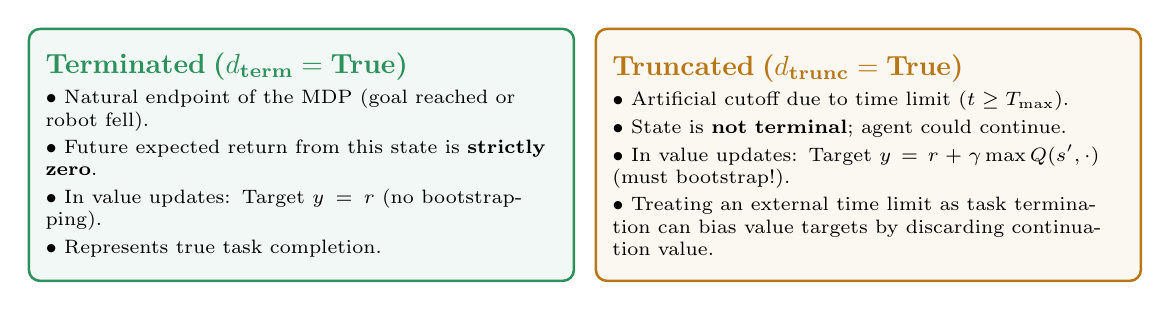
\begin{tikzpicture}[
      box/.style={rounded corners=4pt, text width=6.5cm, minimum height=3.2cm, inner sep=6pt, font=\scriptsize, line width=0.9pt, align=left}
    ]
      % Terminated
      \node[box, draw=islgreen, fill=islgreen!6] at (3.5, 1.7) {
        {\bfseries\color{islgreen}\normalsize Terminated ($d_{\text{term}} = \text{True}$)}\\[3pt]
        $\bullet$ Natural endpoint of the MDP (goal reached or robot fell).\\[2pt]
        $\bullet$ Future expected return from this state is \textbf{strictly zero}.\\[2pt]
        $\bullet$ In value updates: Target $y = r$ (no bootstrapping).\\[2pt]
        $\bullet$ Represents true task completion.
      };

      % Truncated
      \node[box, draw=islgold, fill=islgold!6] at (10.7, 1.7) {
        {\bfseries\color{islgold}\normalsize Truncated ($d_{\text{trunc}} = \text{True}$)}\\[3pt]
        $\bullet$ Artificial cutoff due to time limit ($t \ge T_{\max}$).\\[2pt]
        $\bullet$ State is \textbf{not terminal}; agent could continue.\\[2pt]
        $\bullet$ In value updates: Target $y = r + \gamma \max Q(s', \cdot)$ (must bootstrap!).\\[2pt]
        $\bullet$ Treating an external time limit as task termination can bias value targets by discarding continuation value.
      };
    \end{tikzpicture}
  \par}
\end{frame}

% ==========================================
% SLIDE 7: Code Lens - Minimal Python Loop
% ==========================================
\begin{frame}[fragile]{Code Lens: Inspecting a Tiny MDP in Python}
  \sectionlabel{The canonical environment interaction pattern in examples/week-01}

  \begin{columns}[T,onlytextwidth]
    \column{0.55\textwidth}
      {\small\bfseries\color{islteal} Canonical Environment Loop}\par\vspace{0.06cm}
      {\footnotesize
      \begin{block}{\footnotesize Python Execution Pattern}
\texttt{env = LineWorld(size=5, max\_steps=20)}\\
\texttt{state = env.reset(start=0)}\\
\texttt{done = False; ep\_return = 0.0}\\[3pt]
\texttt{while not done:}\\
\texttt{\quad action = policy(state)}\\
\texttt{\quad res = env.step(action)}\\
\texttt{\quad ep\_return += res.reward}\\
\texttt{\quad state = res.state}\\
\texttt{\quad done = res.terminated or res.truncated}
      \end{block}}

    \column{0.41\textwidth}
      {\small\bfseries\color{islnavy} Key Takeaways}\par\vspace{0.06cm}
      {\footnotesize
      $\bullet$ Three core steps: \textbf{observe $\to$ act $\to$ step}.\\[2pt]
      $\bullet$ Track scalar return $G = \sum r_t$.\\[2pt]
      $\bullet$ Cleanly separate agent decision logic from environment transition logic.\\[2pt]
      $\bullet$ Transparent, zero external dependencies.}
  \end{columns}
\end{frame}

% ==========================================
% SLIDE 8: Failure Modes & Debugging Traps
% ==========================================
\begin{frame}{Failure Modes in MDP Formulation}
  \sectionlabel{Common pitfalls when formulating tasks and evaluating baselines}

  \begin{center}
    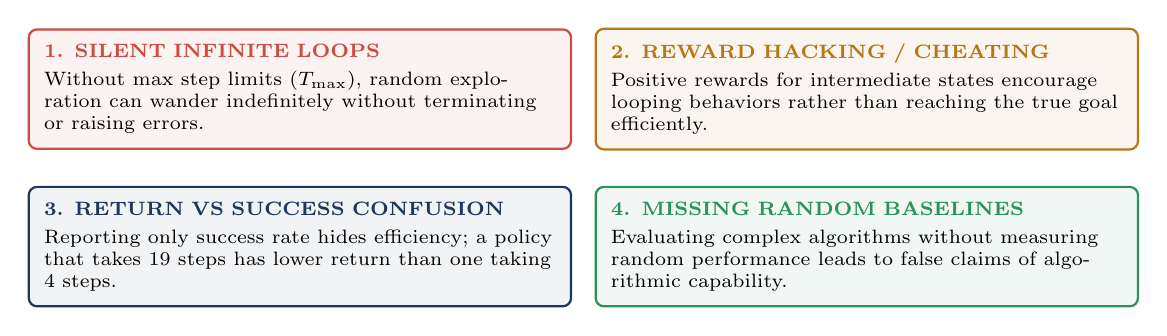
\begin{tikzpicture}[
      card/.style={rounded corners=3pt, text width=6.5cm, minimum height=1.35cm, align=left, inner sep=5.5pt, font=\scriptsize, line width=0.8pt}
    ]
      \node[card, draw=islred, fill=islred!7] at (3.5, 3.3) {
        {\bfseries\color{islred} 1. SILENT INFINITE LOOPS}\\[2pt]
        Without max step limits ($T_{\max}$), random exploration can wander indefinitely without terminating or raising errors.
      };

      \node[card, draw=islgold, fill=islgold!7] at (10.7, 3.3) {
        {\bfseries\color{islgold} 2. REWARD HACKING / CHEATING}\\[2pt]
        Positive rewards for intermediate states encourage looping behaviors rather than reaching the true goal efficiently.
      };

      \node[card, draw=islnavy, fill=islnavy!6] at (3.5, 1.3) {
        {\bfseries\color{islnavy} 3. RETURN VS SUCCESS CONFUSION}\\[2pt]
        Reporting only success rate hides efficiency; a policy that takes 19 steps has lower return than one taking 4 steps.
      };

      \node[card, draw=islgreen, fill=islgreen!7] at (10.7, 1.3) {
        {\bfseries\color{islgreen} 4. MISSING RANDOM BASELINES}\\[2pt]
        Evaluating complex algorithms without measuring random performance leads to false claims of algorithmic capability.
      };
    \end{tikzpicture}
  \end{center}
\end{frame}

% ==========================================
% SLIDE 9: Robotics Horizon Bridge
% ==========================================
\begin{frame}{Robotics Bridge: Formulating Real Systems as MDPs}
  \sectionlabel{Mapping continuous physical robotic systems into the formal MDP framework}

  \begin{columns}[T,onlytextwidth]
    \column{0.48\textwidth}
      {\small\bfseries\color{islnavy} Physical Robot MDP Mapping}\par\vspace{0.08cm}
      {\footnotesize
      $\bullet$ \textbf{State $\mathcal{S}$:} Joint positions $\theta \in \mathbb{R}^7$, velocities $\dot{\theta}$, end-effector pose $T_{ee} \in \text{SE}(3)$, tactile forces.\\[2pt]
      $\bullet$ \textbf{Action $\mathcal{A}$:} Motor torques $\tau \in \mathbb{R}^7$ or delta Cartesian setpoints $\Delta x \in \mathbb{R}^6$.\\[2pt]
      $\bullet$ \textbf{Transitions $\mathcal{P}$:} Governed by rigid body physics, contact dynamics, and motor inertia.}

    \column{0.48\textwidth}
      {\small\bfseries\color{islteal} Reward Engineering in Robotics}\par\vspace{0.08cm}
      {\footnotesize
      $\bullet$ \textbf{Dense Rewards:} Distance to target $-\|x_{\text{ee}} - x_{\text{target}}\|_2$ (smooth gradients, risk of unintended exploits).\\[2pt]
      $\bullet$ \textbf{Sparse Rewards:} $+1$ on successful grasp (unbiased, but difficult exploration).\\[2pt]
      $\bullet$ \textbf{Safety Costs:} Penalty for exceeding joint torque limits or collisions.}
  \end{columns}
\end{frame}

% ==========================================
% SLIDE 10: Quiz Part 1 - Concepts Check
% ==========================================
\begin{frame}{Week 01 Quiz: Core Concepts \& Interaction Loop}
  \sectionlabel{Self-check: verify fundamental understanding of MDPs and baselines}

  \begin{center}
    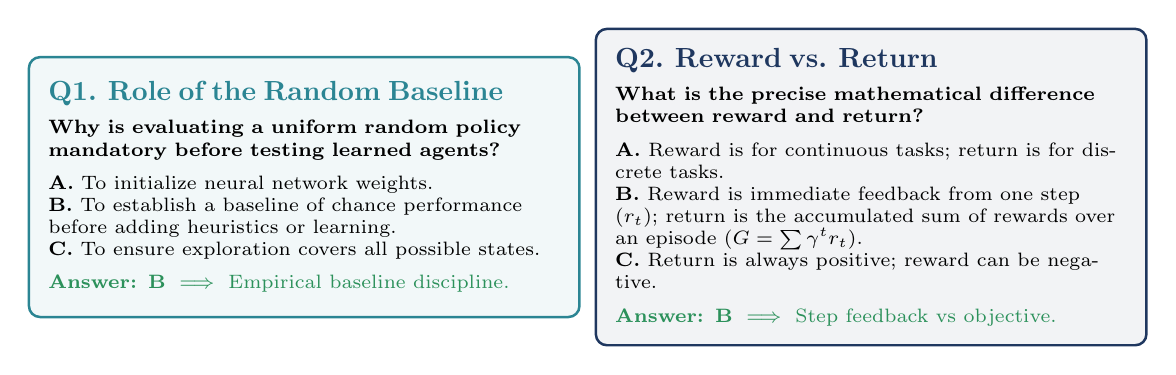
\begin{tikzpicture}[
      qcard/.style={rounded corners=4pt, text width=6.5cm, minimum height=3.3cm, align=left, inner sep=7pt, font=\scriptsize, line width=0.9pt}
    ]
      % Question 1
      \node[qcard, draw=islteal, fill=islteal!6] at (3.5, 1.7) {
        {\bfseries\color{islteal}\normalsize Q1. Role of the Random Baseline}\\[4pt]
        \textbf{Why is evaluating a uniform random policy mandatory before testing learned agents?}\\[4pt]
        \textbf{A.} To initialize neural network weights.\\
        \textbf{B.} To establish a baseline of chance performance before adding heuristics or learning.\\
        \textbf{C.} To ensure exploration covers all possible states.
        \vskip4pt
        {\color{islgreen}\textbf{Answer: B} $\implies$ Empirical baseline discipline.}
      };

      % Question 2
      \node[qcard, draw=islnavy, fill=islnavy!6] at (10.7, 1.7) {
        {\bfseries\color{islnavy}\normalsize Q2. Reward vs. Return}\\[4pt]
        \textbf{What is the precise mathematical difference between reward and return?}\\[4pt]
        \textbf{A.} Reward is for continuous tasks; return is for discrete tasks.\\
        \textbf{B.} Reward is immediate feedback from one step ($r_t$); return is the accumulated sum of rewards over an episode ($G = \sum \gamma^t r_t$).\\
        \textbf{C.} Return is always positive; reward can be negative.
        \vskip4pt
        {\color{islgreen}\textbf{Answer: B} $\implies$ Step feedback vs objective.}
      };
    \end{tikzpicture}
  \end{center}
\end{frame}

% ==========================================
% SLIDE 11: Quiz Part 2 - Rollout Reading & Arithmetic
% ==========================================
\begin{frame}{Week 01 Quiz: Rollout Reading \& Return Arithmetic}
  \sectionlabel{Verify hand-computations for trajectory returns and step costs}

  \begin{center}
    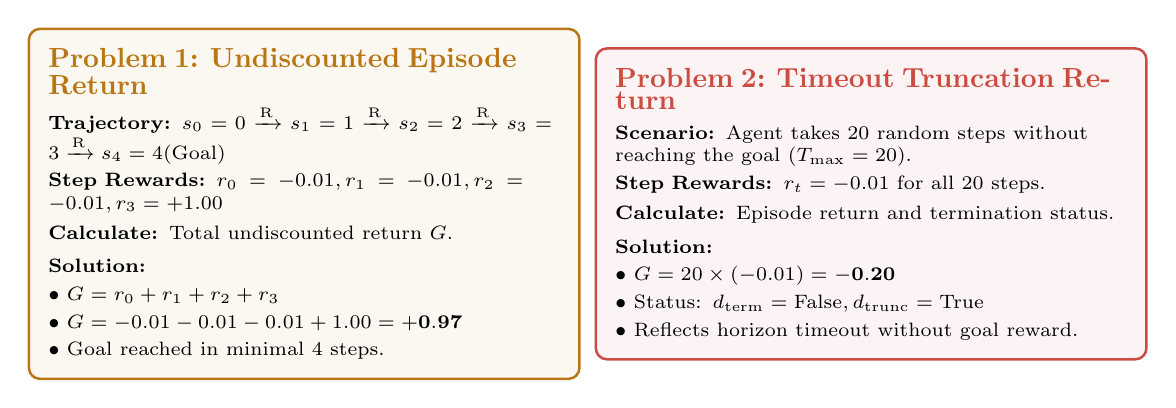
\begin{tikzpicture}[
      qcard/.style={rounded corners=4pt, text width=6.5cm, minimum height=3.3cm, align=left, inner sep=7pt, font=\scriptsize, line width=0.9pt}
    ]
      % Problem 1
      \node[qcard, draw=islgold, fill=islgold!6] at (3.5, 1.7) {
        {\bfseries\color{islgold}\normalsize Problem 1: Undiscounted Episode Return}\\[3pt]
        \textbf{Trajectory:} $s_0=0 \xrightarrow{\text{R}} s_1=1 \xrightarrow{\text{R}} s_2=2 \xrightarrow{\text{R}} s_3=3 \xrightarrow{\text{R}} s_4=4 (\text{Goal})$\\[2pt]
        \textbf{Step Rewards:} $r_0=-0.01, r_1=-0.01, r_2=-0.01, r_3=+1.00$\\[3pt]
        \textbf{Calculate:} Total undiscounted return $G$.\\[4pt]
        \textbf{Solution:}\\[2pt]
        $\bullet$ $G = r_0 + r_1 + r_2 + r_3$\\[2pt]
        $\bullet$ $G = -0.01 - 0.01 - 0.01 + 1.00 = \mathbf{+0.97}$\\[2pt]
        $\bullet$ Goal reached in minimal 4 steps.
      };

      % Problem 2
      \node[qcard, draw=islred, fill=islred!6] at (10.7, 1.7) {
        {\bfseries\color{islred}\normalsize Problem 2: Timeout Truncation Return}\\[3pt]
        \textbf{Scenario:} Agent takes 20 random steps without reaching the goal ($T_{\max}=20$).\\[2pt]
        \textbf{Step Rewards:} $r_t = -0.01$ for all 20 steps.\\[3pt]
        \textbf{Calculate:} Episode return and termination status.\\[4pt]
        \textbf{Solution:}\\[2pt]
        $\bullet$ $G = 20 \times (-0.01) = \mathbf{-0.20}$\\[2pt]
        $\bullet$ Status: $d_{\text{term}}=\text{False}, d_{\text{trunc}}=\text{True}$\\[2pt]
        $\bullet$ Reflects horizon timeout without goal reward.
      };
    \end{tikzpicture}
  \end{center}
\end{frame}

% ==========================================
% SLIDE 12: Quiz Part 3 - Diagnostics & Traps
% ==========================================
\begin{frame}{Week 01 Quiz: Diagnostics \& Practical Traps}
  \sectionlabel{Key practical questions every RL practitioner must master}

  \begin{center}
    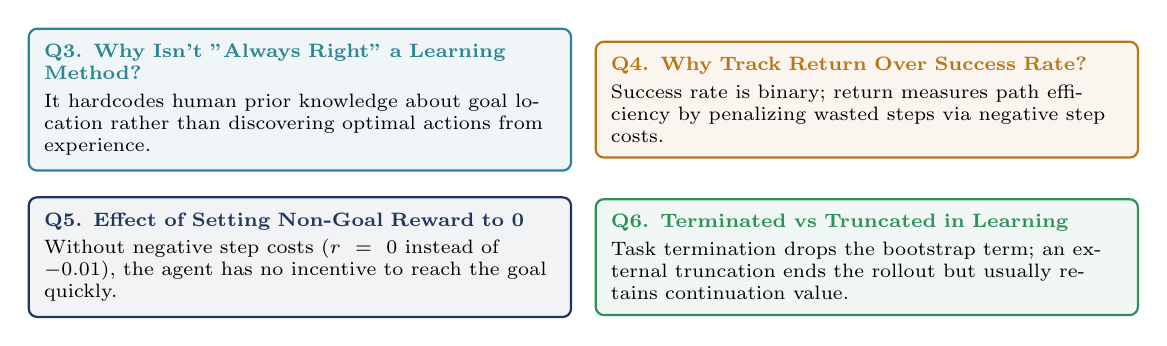
\begin{tikzpicture}[
      card/.style={rounded corners=3pt, text width=6.5cm, minimum height=1.35cm, align=left, inner sep=5.5pt, font=\scriptsize, line width=0.8pt}
    ]
      \node[card, draw=islteal, fill=islteal!7] at (3.5, 3.3) {
        {\bfseries\color{islteal} Q3. Why Isn't "Always Right" a Learning Method?}\\[2pt]
        It hardcodes human prior knowledge about goal location rather than discovering optimal actions from experience.
      };

      \node[card, draw=islgold, fill=islgold!7] at (10.7, 3.3) {
        {\bfseries\color{islgold} Q4. Why Track Return Over Success Rate?}\\[2pt]
        Success rate is binary; return measures path efficiency by penalizing wasted steps via negative step costs.
      };

      \node[card, draw=islnavy, fill=islnavy!6] at (3.5, 1.3) {
        {\bfseries\color{islnavy} Q5. Effect of Setting Non-Goal Reward to 0}\\[2pt]
        Without negative step costs ($r=0$ instead of $-0.01$), the agent has no incentive to reach the goal quickly.
      };

      \node[card, draw=islgreen, fill=islgreen!7] at (10.7, 1.3) {
        {\bfseries\color{islgreen} Q6. Terminated vs Truncated in Learning}\\[2pt]
        Task termination drops the bootstrap term; an external truncation ends the rollout but usually retains continuation value.
      };
    \end{tikzpicture}
  \end{center}
\end{frame}

\end{document}
